\chapter{Background}

\section{Sentiment Analysis}
In the nutshell, sentiment analysis is to determine whether the opinion about a specific product, event, organization is positive or negative.  
\subsection{The need for sentiment analysis}
Every business need feedback from customer. Feedback help company know their product strength and weakness, drive business strategy. For example, fix the flaw in product, target new customer segment or halt a campaign. Traditional, company would survey their customer to collect feedback.  The feedback collected from direct survey are limited for many reason, such as low population. 

With the growth of social network and e-commerce, more and more people post their opinion online via blog, social network (Facebook, Twitter), e-commerce site (Amazon, eBay). Company want to take advantage of these data. Thus, a automate system to analysis opinion are in demand. 
            
\subsection{The challenges}
Lorem ipsum dolor sit amet, consectetur adipiscing elit, sed do eiusmod tempor incididunt ut labore et dolore magna aliqua. Ut enim ad minim veniam, quis nostrud exercitation ullamco laboris nisi ut aliquip ex ea commodo consequat. Duis aute irure dolor in reprehenderit in voluptate velit esse cillum dolore eu fugiat nulla pariatur. Excepteur sint occaecat cupidatat non proident, sunt in culpa qui officia deserunt mollit anim id est laborum.

\subsection{Different levels in sentiment analysis}
\subsubsection{Document-level}
Document-level sentiment analysis is to determine whether a document (usually a full review) about a specific entity (a product, location, service, ...) is positive or negative. For example, \cite{pang2002thumbs} perform document-level sentiment analysis on movies review data.
\subsubsection{Sentence-level}
Sentence-level sentiment analysis is to determine whether a sentence expressed positive, negative. In this thesis, we focus our study on sentence-level sentiment analysis \cite{liu2012sentiment}. 
\subsubsection{Aspect-level}
Aspect-level  sentiment analysis purpose is to determine opinion, whether positive or negative, against specific aspect of entity \cite{liu2012sentiment}. 

\section{Feedforward neural network}
Feedforward neural network is a network whether unit in the graph does not form a cycle \cite{Goodfelloetal2016}. 

Each feedforward neural network consist at least one input layer, one output layer. Each layer contain one or more neurons (network nodes). Each neuron consist of a linear activation or non-linear activation function. 

Each node have an activation function. There are two type of activation function: Linear and non-linear. 

Example of linear function: \\
\[f(x) = Wx + b \]

Example of non-linear function: \\
\[f(x) = tanh(x) \]
\[f(x) =\frac{1}{1+e^{-x}} \]

\subsection{Single-layer perceptron}
Singlelayer perceptron is a feedforward neural network only have one input layer and one output layer of neuron unit (See fig \ref{fig:singleperceptron}). Singlelayer perceptron cannot solve some problem such as XOR.
\begin{figure}[H]
	\centering
	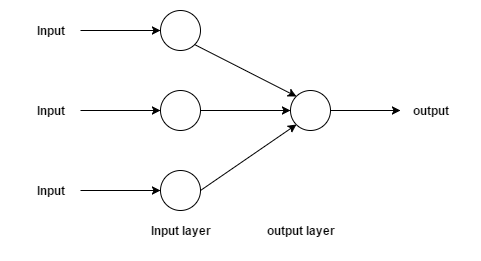
\includegraphics[width=0.7\linewidth]{../figure/singleperceptron}
	\caption[Single-layer Perceptron]{Single-layer Perceptron}
	\label{fig:singleperceptron}
\end{figure}



\subsection{Multi-layer perceptron}
Multilayer perceptron (MLP) is a feedforward neural network consist of 2 or more layer (See fig \ref{fig:multilayerperceptron}). First layer called input layer. Last layer called output layer. All layer between input and output layer are hidden layer. A series of linear function is equal to 2 layer perceptron. Hence, MLP always contain non-linear activation function. In MLP, every unit of previous layer connect to all unit in next layer.

\begin{figure}[H]
	\centering
	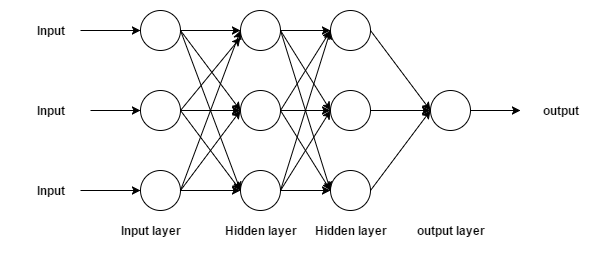
\includegraphics[width=0.7\linewidth]{../figure/multilayerperceptron}
	\caption[Multi-layer Perceptron]{Multi-layer Perceptron}
	\label{fig:multilayerperceptron}
\end{figure}

\subsection{Forward pass}
Forward pass, or forward propagation, is a process which information from input x flow through the network to output y. In MLP forward pass, an input x is feed through first layer, also known as input layer. Output from first layer is use as input for second layer, and so on until it reach last layer, output layer. Output from output layer are output of MLP. 

For example: a MLP with 4 activation function: $f(x)$, $g(x)$, $h(x)$, $k(x)$. With $f(x)$ is input layer, $k(x)$ is output layer, and $g(x), h(x)$ are hidden layers .With input $x$, then MLP has output $ y = k(h(g(f(x))))$.

\subsection{Cost function}
Cost function $J(\theta)$  is a measurement how far predicted  $\hat y$ from expected label $y$. When our model predict exactly the labeled output, then cost function is zero. The problem is to minimize the cost function. Cost function of MLP dependent on output layer.

For most of our experiment, we would use softmax output layer and cross-entropy loss function.
\subsection{Backward pass}





\section{Convolution Neural Network}
Lorem ipsum dolor sit amet, consectetur adipiscing elit, sed do eiusmod tempor incididunt ut labore et dolore magna aliqua. Ut enim ad minim veniam, quis nostrud exercitation ullamco laboris nisi ut aliquip ex ea commodo consequat. Duis aute irure dolor in reprehenderit in voluptate velit esse cillum dolore eu fugiat nulla pariatur. Excepteur sint occaecat cupidatat non proident, sunt in culpa qui officia deserunt mollit anim id est laborum.
\subsection{Architect}
Lorem ipsum dolor sit amet, consectetur adipiscing elit, sed do eiusmod tempor incididunt ut labore et dolore magna aliqua. Ut enim ad minim veniam, quis nostrud exercitation ullamco laboris nisi ut aliquip ex ea commodo consequat. Duis aute irure dolor in reprehenderit in voluptate velit esse cillum dolore eu fugiat nulla pariatur. Excepteur sint occaecat cupidatat non proident, sunt in culpa qui officia deserunt mollit anim id est laborum.
\subsection{Back propagation}
Lorem ipsum dolor sit amet, consectetur adipiscing elit, sed do eiusmod tempor incididunt ut labore et dolore magna aliqua. Ut enim ad minim veniam, quis nostrud exercitation ullamco laboris nisi ut aliquip ex ea commodo consequat. Duis aute irure dolor in reprehenderit in voluptate velit esse cillum dolore eu fugiat nulla pariatur. Excepteur sint occaecat cupidatat non proident, sunt in culpa qui officia deserunt mollit anim id est laborum.
\section{Recurrent Neural Network}
Lorem ipsum dolor sit amet, consectetur adipiscing elit, sed do eiusmod tempor incididunt ut labore et dolore magna aliqua. Ut enim ad minim veniam, quis nostrud exercitation ullamco laboris nisi ut aliquip ex ea commodo consequat. Duis aute irure dolor in reprehenderit in voluptate velit esse cillum dolore eu fugiat nulla pariatur. Excepteur sint occaecat cupidatat non proident, sunt in culpa qui officia deserunt mollit anim id est laborum.
\subsection{RNN}
Lorem ipsum dolor sit amet, consectetur adipiscing elit, sed do eiusmod tempor incididunt ut labore et dolore magna aliqua. Ut enim ad minim veniam, quis nostrud exercitation ullamco laboris nisi ut aliquip ex ea commodo consequat. Duis aute irure dolor in reprehenderit in voluptate velit esse cillum dolore eu fugiat nulla pariatur. Excepteur sint occaecat cupidatat non proident, sunt in culpa qui officia deserunt mollit anim id est laborum.
\subsection{LSTM}
Lorem ipsum dolor sit amet, consectetur adipiscing elit, sed do eiusmod tempor incididunt ut labore et dolore magna aliqua. Ut enim ad minim veniam, quis nostrud exercitation ullamco laboris nisi ut aliquip ex ea commodo consequat. Duis aute irure dolor in reprehenderit in voluptate velit esse cillum dolore eu fugiat nulla pariatur. Excepteur sint occaecat cupidatat non proident, sunt in culpa qui officia deserunt mollit anim id est laborum.
\subsection{Back propagation}
Lorem ipsum dolor sit amet, consectetur adipiscing elit, sed do eiusmod tempor incididunt ut labore et dolore magna aliqua. Ut enim ad minim veniam, quis nostrud exercitation ullamco laboris nisi ut aliquip ex ea commodo consequat. Duis aute irure dolor in reprehenderit in voluptate velit esse cillum dolore eu fugiat nulla pariatur. Excepteur sint occaecat cupidatat non proident, sunt in culpa qui officia deserunt mollit anim id est laborum.
\section{Distributed Representations of Words}
\subsection{Definition}
Lorem ipsum dolor sit amet, consectetur adipiscing elit, sed do eiusmod tempor incididunt ut labore et dolore magna aliqua. Ut enim ad minim veniam, quis nostrud exercitation ullamco laboris nisi ut aliquip ex ea commodo consequat. Duis aute irure dolor in reprehenderit in voluptate velit esse cillum dolore eu fugiat nulla pariatur. Excepteur sint occaecat cupidatat non proident, sunt in culpa qui officia deserunt mollit anim id est laborum.
\subsection{work2vec}
Lorem ipsum dolor sit amet, consectetur adipiscing elit, sed do eiusmod tempor incididunt ut labore et dolore magna aliqua. Ut enim ad minim veniam, quis nostrud exercitation ullamco laboris nisi ut aliquip ex ea commodo consequat. Duis aute irure dolor in reprehenderit in voluptate velit esse cillum dolore eu fugiat nulla pariatur. Excepteur sint occaecat cupidatat non proident, sunt in culpa qui officia deserunt mollit anim id est laborum.
\subsection{Glove}
Lorem ipsum dolor sit amet, consectetur adipiscing elit, sed do eiusmod tempor incididunt ut labore et dolore magna aliqua. Ut enim ad minim veniam, quis nostrud exercitation ullamco laboris nisi ut aliquip ex ea commodo consequat. Duis aute irure dolor in reprehenderit in voluptate velit esse cillum dolore eu fugiat nulla pariatur. Excepteur sint occaecat cupidatat non proident, sunt in culpa qui officia deserunt mollit anim id est laborum.
\subsection{Different methods to produce word embedding}
Lorem ipsum dolor sit amet, consectetur adipiscing elit, sed do eiusmod tempor incididunt ut labore et dolore magna aliqua. Ut enim ad minim veniam, quis nostrud exercitation ullamco laboris nisi ut aliquip ex ea commodo consequat. Duis aute irure dolor in reprehenderit in voluptate velit esse cillum dolore eu fugiat nulla pariatur. Excepteur sint occaecat cupidatat non proident, sunt in culpa qui officia deserunt mollit anim id est laborum.
\section{Parse tree in NLP}
Lorem ipsum dolor sit amet, consectetur adipiscing elit, sed do eiusmod tempor incididunt ut labore et dolore magna aliqua. Ut enim ad minim veniam, quis nostrud exercitation ullamco laboris nisi ut aliquip ex ea commodo consequat. Duis aute irure dolor in reprehenderit in voluptate velit esse cillum dolore eu fugiat nulla pariatur. Excepteur sint occaecat cupidatat non proident, sunt in culpa qui officia deserunt mollit anim id est laborum.
\subsection{Constituency Parse Tree}
Lorem ipsum dolor sit amet, consectetur adipiscing elit, sed do eiusmod tempor incididunt ut labore et dolore magna aliqua. Ut enim ad minim veniam, quis nostrud exercitation ullamco laboris nisi ut aliquip ex ea commodo consequat. Duis aute irure dolor in reprehenderit in voluptate velit esse cillum dolore eu fugiat nulla pariatur. Excepteur sint occaecat cupidatat non proident, sunt in culpa qui officia deserunt mollit anim id est laborum.
\subsection{Dependency Parse Tree}
Lorem ipsum dolor sit amet, consectetur adipiscing elit, sed do eiusmod tempor incididunt ut labore et dolore magna aliqua. Ut enim ad minim veniam, quis nostrud exercitation ullamco laboris nisi ut aliquip ex ea commodo consequat. Duis aute irure dolor in reprehenderit in voluptate velit esse cillum dolore eu fugiat nulla pariatur. Excepteur sint occaecat cupidatat non proident, sunt in culpa qui officia deserunt mollit anim id est laborum.
\section{Recursive Neural Network}
Lorem ipsum dolor sit amet, consectetur adipiscing elit, sed do eiusmod tempor incididunt ut labore et dolore magna aliqua. Ut enim ad minim veniam, quis nostrud exercitation ullamco laboris nisi ut aliquip ex ea commodo consequat. Duis aute irure dolor in reprehenderit in voluptate velit esse cillum dolore eu fugiat nulla pariatur. Excepteur sint occaecat cupidatat non proident, sunt in culpa qui officia deserunt mollit anim id est laborum.
\subsection{RNN: Recursive Neural Network}
Lorem ipsum dolor sit amet, consectetur adipiscing elit, sed do eiusmod tempor incididunt ut labore et dolore magna aliqua. Ut enim ad minim veniam, quis nostrud exercitation ullamco laboris nisi ut aliquip ex ea commodo consequat. Duis aute irure dolor in reprehenderit in voluptate velit esse cillum dolore eu fugiat nulla pariatur. Excepteur sint occaecat cupidatat non proident, sunt in culpa qui officia deserunt mollit anim id est laborum.
\subsection{MV-RNN: Matrix-Vector RNN}
Lorem ipsum dolor sit amet, consectetur adipiscing elit, sed do eiusmod tempor incididunt ut labore et dolore magna aliqua. Ut enim ad minim veniam, quis nostrud exercitation ullamco laboris nisi ut aliquip ex ea commodo consequat. Duis aute irure dolor in reprehenderit in voluptate velit esse cillum dolore eu fugiat nulla pariatur. Excepteur sint occaecat cupidatat non proident, sunt in culpa qui officia deserunt mollit anim id est laborum.
\subsection{RNTN:Recursive Neural Tensor}
Lorem ipsum dolor sit amet, consectetur adipiscing elit, sed do eiusmod tempor incididunt ut labore et dolore magna aliqua. Ut enim ad minim veniam, quis nostrud exercitation ullamco laboris nisi ut aliquip ex ea commodo consequat. Duis aute irure dolor in reprehenderit in voluptate velit esse cillum dolore eu fugiat nulla pariatur. Excepteur sint occaecat cupidatat non proident, sunt in culpa qui officia deserunt mollit anim id est laborum. Network
\section{Programming Framework}
\subsubsection{RNTN:Recursive Neural Tensor}
Lorem ipsum dolor sit amet, consectetur adipiscing elit, sed do eiusmod tempor incididunt ut labore et dolore magna aliqua. Ut enim ad minim veniam, quis nostrud exercitation ullamco laboris nisi ut aliquip ex ea commodo consequat. Duis aute irure dolor in reprehenderit in voluptate velit esse cillum dolore eu fugiat nulla pariatur. Excepteur sint occaecat cupidatat non proident, sunt in culpa qui officia deserunt mollit anim id est laborum. Network
\subsection{Torch}
Torch \footnote{http://torch.ch/} is Lua scientific computing framework. Torch support high performing matrix calculation via multi-dimensional array call Tensor. Torch are built with C/C++, CUDA backend. Torch author choose Lua because Lua works well with C/C++ \cite{collobert2011torch7}.  Thus, Torch is high performing and support GPU. Torch have neural network package (nn) package. Computation graph must be define before forward pass. 
A simple, single linear layer network can be easily defined with few line of code (see listing \ref{lst:torchlinear}).

\begin{lstlisting}[caption={Simple linear layer in Torch},label={lst:torchlinear}, language={[5.1]Lua}]
-- simple y = Ax + b linear layer
l = nn.Linear(2,3)
-- forward pass
x = torch.Tensor(2)
y = l:forward(x) -- vector dimension of 3
\end{lstlisting}

However, when a model need multiple module, such as multilayer perceptron (MLP), these module must be put into container. Figure \ref{fig:nncontainer} illustrates on function of each nn container . In order to construct two-layer perception (eq \ref{eq:mlp}), linear, tanh and softmax module must be packed into sequential module (see listing \ref{lst:torchmlp}).

\begin{equation}
\label{eq:mlp}
\begin{aligned}
&h = tanh(W_1*x + b_1) \\
&y = softmax(W_2*h + b2)
\end{aligned}
\end{equation}


\begin{lstlisting}[caption={MLP in Torch},label={lst:torchmlp}, language={[5.1]Lua}]
model = nn.Sequential()
model:add(nn.Linear(2,3))
model:add(nn.Tanh())
model:add(nn.Linear(3,5))
model:add(nn.SoftMax())
-- forward
x = torch.Tensor(2)
y = model:forward(x)
\end{lstlisting}

Torch provide nngraph package support build more complicate model. For example, define MLP in (eq \ref{eq:mlp}) use nngraph (see listing \ref{lst:torchnngraph})

\begin{lstlisting}[caption={MLP using nngraph},label={lst:torchnngraph}, language={[5.1]Lua}]
model = nn.Sequential()
model:add(nn.Linear(2,3))
model:add(nn.Tanh())
model:add(nn.Linear(3,5))
model:add(nn.SoftMax())
-- forward
x = torch.Tensor(2)
y = model:forward(x)
\end{lstlisting}

Sample code on training a model, see Appendix \ref{lst:torchtrain}

\subsection{Theano}
Theano \footnote{\url{http://deeplearning.net/software/theano/}} is a deep learning library on Python. It basic function is similar to Torch: matrix calculation, support GPU. Theano is define-and-run schema, which a computer graph must be built before it is executed.

\begin{lstlisting}[caption={Define function in Theano},label={lst:theanof}, language={python}]
x = T.dmatrix('x')
y = T.dmatrix('y')
z = x + y
f = function([x, y], z)
f([[1, 1], [2, 2]], [[3, 3], [4, 4]])
# result [[4, 4], [6, 6]]
\end{lstlisting}

Comparing to Torch7, Theano are slower on most benchmark \cite{collobert2011torch7}. Theano does not provide nice template like linear layer. Thus, model must be defined from equation. It give researcher more control over mathematics aspect but cause more trouble for beginner. A sample code for MLP \ref{lst:theanomlp}. One more problem is that the 'define-and-run' scheme does not suitable for recursive neural network due to recompile the computation graph each training sample take time. 

\subsection{Pytorch}
PyTorch uses same backend as Torch. However, PyTorch specially designed for Python. Pytorch have pre-define module (Linear layer, Convolution layer) like Torch. However, Pytorch does not require to pack model into container. In Pytorch a network are defined in forward-pass thanks to Dynamic Neural Networks feature. Therefore, user can use Python control flow to define a network. For example, one can use for loop to run recurrent neural network (see listing \ref{lst:pytorchrnn}) .The features allows us to implement Recursive Neural Network for NLP, which the network change for every sample, much more easier. 

\begin{lstlisting}[caption={RNN},label={lst:pytorchrnn}, language={python}]
import torch
import torch.nn as nn
rnn = nn.RNNCell(10, 20)
seq_len = 10
input_dim = 100
hidden_dim = 150
input = Variable(torch.randn(seq_len, 1, input_dim))
hx = Variable(torch.zeros(1, hidden_dim))
output = []
for i in range(6):
    hx = rnn(input[i], hx)
    output.append(hx)
\end{lstlisting}

We also implement treelstm from original Torch7 \footnote{\url{https://github.com/stanfordnlp/treelstm}} sentiment classification task in PyTorch and publish on Github \footnote{\url{https://github.com/ttpro1995/TreeLSTMSentiment}}.   

We choose PyTorch because: 
\begin{itemize}
	\item Dynamic Neural Networks feature works well on data sequence with different length
	\item Intuitive framework
	\item Easy to install and run on CUDA
\end{itemize}



